\documentclass{article}
\usepackage{listings}
\usepackage{color}
\usepackage{graphicx}
\definecolor{codegreen}{rgb}{0,0.6,0}
\definecolor{codegray}{rgb}{0.5,0.5,0.5}
\definecolor{codepurple}{rgb}{0.58,0,0.82}
\definecolor{backcolour}{rgb}{0.95,0.95,0.92}
 
\lstdefinestyle{CodeStyle}{
    backgroundcolor=\color{backcolour},   
    commentstyle=\color{codegreen},
    keywordstyle=\color{magenta},
    numberstyle=\tiny\color{codegray},
    stringstyle=\color{codepurple},
    basicstyle=\footnotesize,
    breakatwhitespace=false,
    breaklines=true,
    captionpos=b,
    keepspaces=true,
    numbers=left,
    numbersep=5pt,
    showspaces=false,
    showstringspaces=false,
    showtabs=false,
    tabsize=2
}

\title{VioletUML Development Guide}
\date{2016-11-05}
\author{roughtomato}

\begin{document}
  \pagenumbering{gobble}
  \maketitle
  \newpage
  \pagenumbering{arabic}

\section{Getting started with VioletUML}
\subsection{Building VioletUML}

In order to create clean development build you'll have to comment out few lines due to some broken functionality in modules responsible for
building executable for specific platform namely 'violetproduct-exe' and 'violetproduct-web' which are causing compilation errors.
Working version should already be at origin/master of this VioletUML although this problem might return in the future with other modules.
Related issue 32. You'll need to edit pom.xml in your project main directory and comment out fallowing lines making it look like this:
\begin{lstlisting}[language=XML]
<modules>
	<module>violet-framework</module>
	<module>violetplugin-activitydiagram</module>
	<module>violetplugin-communicationdiagram</module>
	<module>violetplugin-objectdiagram</module>
	<module>violetplugin-sequecnediagram</module>
	<module>violetplugin-statediagram</module>
	<module>violetplugin-usecasediagram</module>
	<module>violetplugin-swing</module>
	<!--<module>violetproduct-jnlp</module> -->
	<!--<module>violetproduct-exe</module> -->
	<!--<module>violetproduct-rpm</module> -->
	<module>violetproduct-deb</module>
	<!--<module>violetproduct-web</module> -->
\end{lstlisting}

You can probably already notice common theme of how functionality is arranged in this project. We will touch on this subject in the next subsection.
For now you should be able to run maven clean build.
\begin{lstlisting}
	mvn clean install
\end{lstlisting}
Maven should finish building with no errors.

Congratulations! You now have working binaries of VioletUML.

\subsection{Building exe module}

On how to enable or disable modules see above previous
The "exe" module in violetUML require additional 32bit libraries:

- lib32z1\newline
- lib32curses\newline
- lib-ncurses5\newline


\subsection{Code style}

Whole project is written in certain code style convention, we appritiate keeping it unified for readability sake.

Classes and methods :
\begin{lstlisting}
public class SomeClass {

    private String somePrivateString;

    public SomeClass() {
      //some content
    }

    public void someMethod(int someIntager) {
      //some content
    }
}
\end{lstlisting}

As you can see. Camel back names are preferred. Only exceptions should be taken into consideration with very verbose names (which sometimes
can't be avoided) e.g. this\_is\_very\_verbose\_yet\_descriptive\_name. Like for example methods in Selenium framework.\newline
- Two spaces are used as intend inside classes/methods.\newline
- Opening bracket should be in the same line as class/method name.\newline
- Class names should start with capital letter but methods and variables should start with lowercase.\newline

\begin{lstlisting}
 ...
  SomeClass someClassVar = new SomeClass();
  
  for(SomeOtherClass iterateVar : someClassVar.getAll()) {
    iterateVar.doSomething();
    if((iterateVar.getSmth() == 0) && (iterateVar.check() < 1))
    {
      //do something
    }
  }
  
 ...
\end{lstlisting}

Inside methods two space rule still applies.\newline
- declarations of objects should have one line before some more complex logic appear.\newline
- loops operate on the same rule as methods.\newline
- control flow (if, else, else if) should have braces beginning within new line.\newline
- multiple comparisons should be within additional parasynthesis for readability sake.\newline

\subsection{Violet UI}

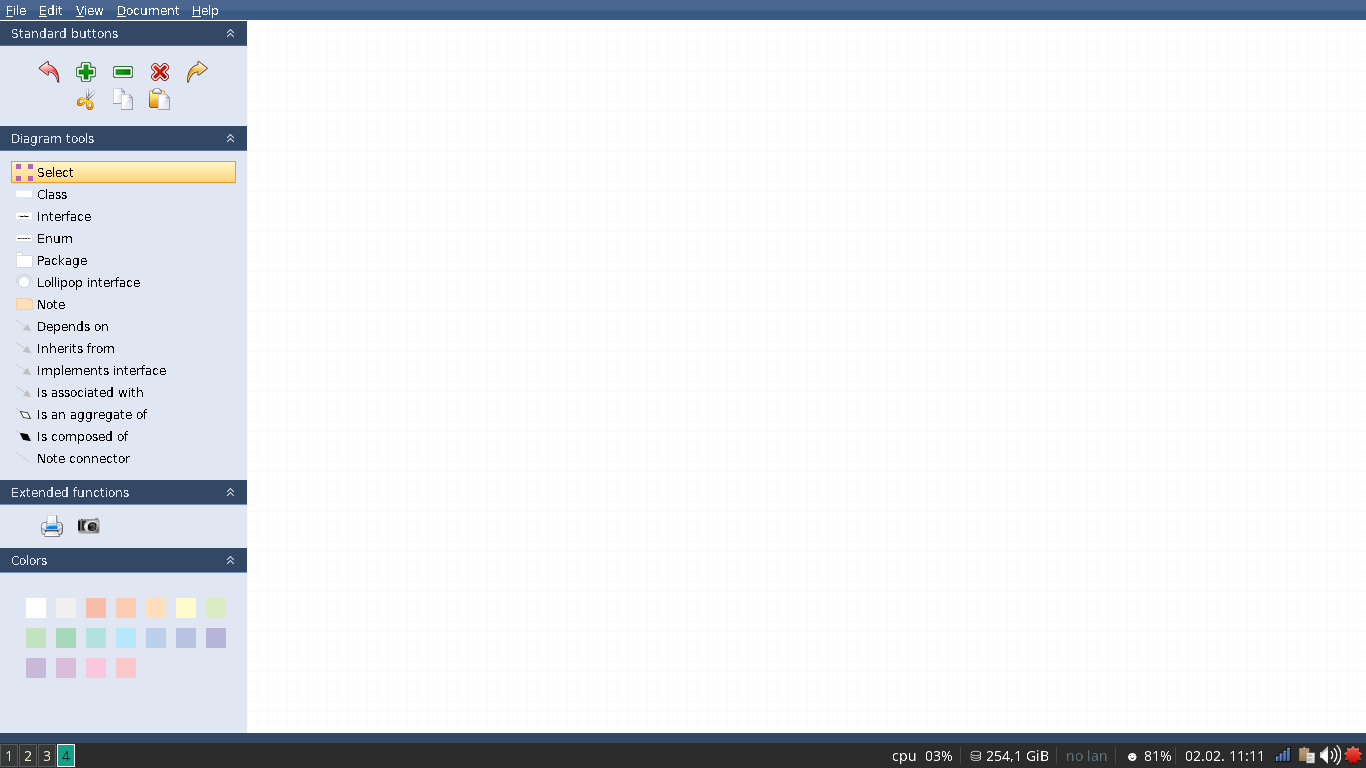
\includegraphics{assets/violetUI}

VioletUML class diagram view. On the top menu we have functionality responsible for saving, starting new file, closing program, editing, undo and redo.
On the left there are diagram specific tools (violetplugin-*)

\subsection{Folder structure}

violet-framework/ is the core structure of this application. You can find here :\newline\newline
- bean injection framework (which is used for loading plugins)\newline
- graphics which is responsible for front end part of the application like overall layout.\newline
- plugin loader\newline
- swingextention that consists mostly of definitions for basic UI elements\newline
- theme is responsible for holding information about layout colors\newline

violetplugin-*/ those folders beginning with violet and followed with plugin means certain functionality
package. e.g. activitydiagram holds logic responsible for everything related to activity diagram.

violetproduct-*/ here you can find binaries after compilation is successful
where "*" means respective format for those binaries.

\subsection{Known issues}

TBA

\subsection{TODO for future releases}
As you probably noticed VioletUML is *slightly* bloated. If you have some spare time
everybody would benefit from overall simplification of core functionalities.
Maybe introducing MV* pattern in order to separate business logic from frontend would be a good idea.
Although it might be very difficult to accomplish.

\subsection{Change log}

Changes from 02.2017 :

- overall refactoring and small code quality improvements \newline
- created this documentation\newline
- added common relation edge\newline
- added safe delete\newline
- added possibility of using html tags\newline
- added full screen capabilities\newline
- added shortcuts that weren't previously defined\newline
- added integration with google drive                        \#958eedc\newline
- added search functionality                                 \#983df43\newline
- added history panel\newline
- added dragging capability to workspace                     \#8896f34\newline
- added detection of duplicate names                         \#0236666\newline
- fixed copy \& cut behavior                                  \#838d94e\newline


\subsection{Special Thanks}
I would like to say thank you for people who helped immensely with making those changes possible.

Special thanks go to : \newline\newline
@NdV66 for help with merging pull requests, code review and releasing final stable version of this software.\newline
@orchowski for help with merging pull requests and code reviews.\newline
@KrystianDziedziola for help with integration.\newline
@bartoszsledz for testing and bug reporting.\newline
\newline
And last but not least\newline
@abizukojc for help with people management, merging pull requests, preparing release, code review and bug fixing.\newline
\newline
Thank you for helping me not to lose all of my sanity.\newline

\end{document}
